\chapter{Database Design}

\section{Entities, Attributes and Relationships}
The database, called a bank, will have two tables, one called accounts and the other called
customer. Each will hold information about either the account or the customer. The two
tables will be linked through a foreign key. The customer table has the following fields:\\
\begin{figure}[H]
\centering
\caption{account user table}
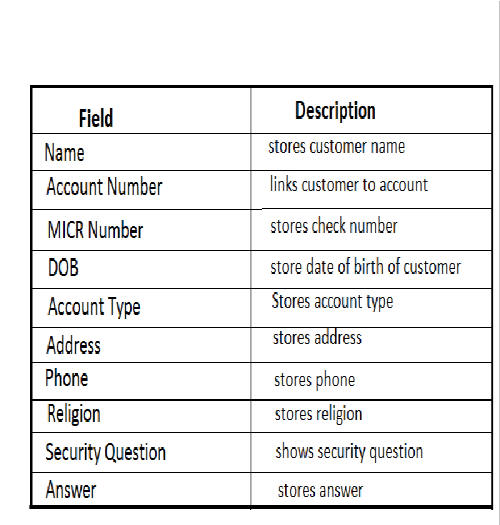
\includegraphics[scale=.5]{./accountUserTable.png}
\\[0.2in]
\label{fig:account user table}
\end{figure}
Since one customer can have many accounts, We thought it only right to insert a foreign key
acc\_id into the customer table. In addition, instead of having fields such as date created and
date closed, I simply use the active field to check if the account is active or not. This will
enable us to focus more on the programming than on particulars of the database.\\
\thispagestyle{fancy}

\section{Identify Major entities, attributes and relationships}
\begin{itemize}
\item User registration for online banking if not register.
\item Adding Beneficiary account by customer using entity called Acconts.
\item Transferring amount to the local customer account number using Transfer entity
which stores the details of transaction.
\item Customer can check all transactions made with their account in their Transaction
details using Transaction Entity or table.
\item Customer can check their account statement within a date range.
\end{itemize}

\thispagestyle{fancy}

\section{ER Schema}
\begin{figure}[H]
\centering
\caption{ERD}
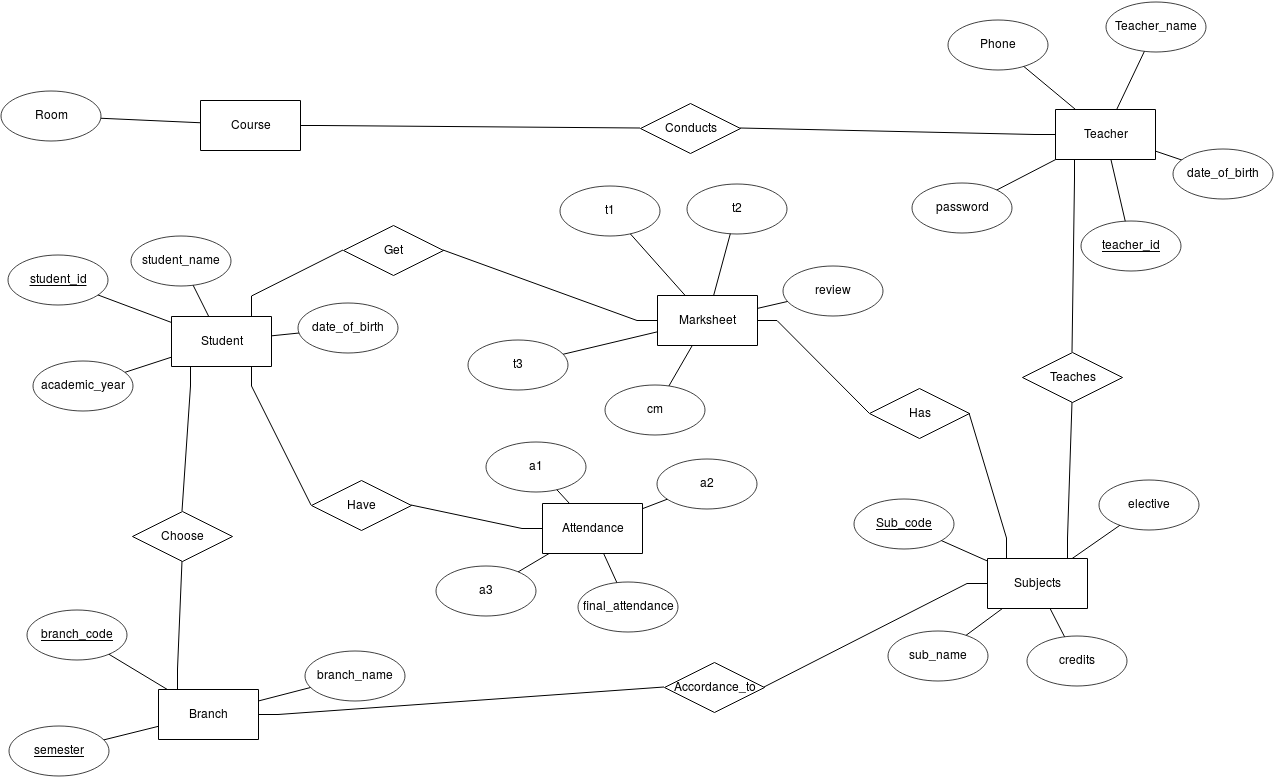
\includegraphics[scale=.5]{./erd.png}
\\[0.2in]
\label{fig:ER diagram}
\end{figure}

\thispagestyle{fancy}

\section{Relational Schema}
\begin{figure}[H]
\centering
\caption{Relational Schema}
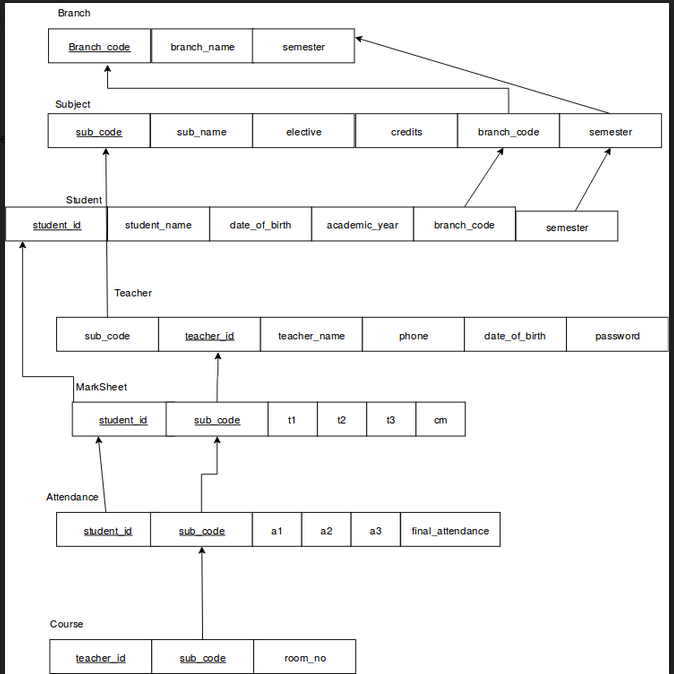
\includegraphics[scale=.5]{./rs.png}
\\[0.2in]
\label{fig:Relational Schema}
\end{figure}

\thispagestyle{fancy}